\documentclass[convert={density=300,size=300x300,outfile=\jobname.png}]{standalone}

\usepackage{tikz}
\usetikzlibrary{automata,calc,trees,positioning,arrows,chains,shapes.geometric,%
decorations.pathreplacing,decorations.pathmorphing,shapes,%
matrix,shapes.symbols,plotmarks,decorations.markings,shadows}

\begin{document}

\begin{tikzpicture}[scale=1]
\draw[->] (-0.5,0)--(5,0) node[right] {$x$};
\node[below] at (0,0) {$a$};
\node[below] at (4.5,0) {$b$};
\draw [red, thick] plot [smooth] coordinates { 
	(0.0, 0.20) 
	(0.5, 0.80) 
	(1.0, 1.30)
	(1.5, 1.70)
	(2.0, 2.00)
	(2.5, 2.20)
	(3.0, 2.30)
	(3.5, 2.30)
	(4.0, 2.10)	
	(4.5, 1.80)
};
\draw [black, fill=gray, opacity=0.3] (0.0, 0.00) -- (0.0, 0.20);
\draw [black, fill=gray, opacity=0.3] (4.5, 0.00) -- (4.5, 1.80);
\end{tikzpicture}
%\caption{Left Riemann Sum}

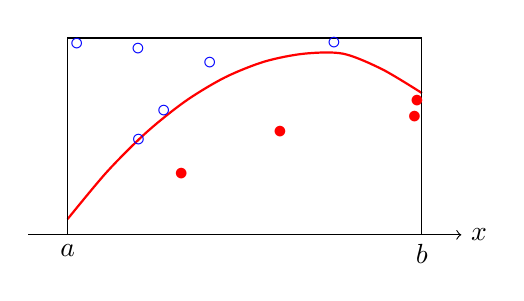
\begin{tikzpicture}[scale=1]
\draw[->] (-0.5,0)--(5,0) node[right] {$x$};
\node[below] at (0,0) {$a$};
\node[below] at (4.5,0) {$b$};
\draw [red, thick] plot [smooth] coordinates { 
	(0.0, 0.20) 
	(0.5, 0.80) 
	(1.0, 1.30)
	(1.5, 1.70)
	(2.0, 2.00)
	(2.5, 2.20)
	(3.0, 2.30)
	(3.5, 2.30)
	(4.0, 2.10)	
	(4.5, 1.80)
};
\draw [black] (0.0, 0.00) rectangle (4.5, 2.50);


\node[red]  at (2.69777,    1.29625)  {$\bullet$};
\node[red]  at (1.44549,    0.764894) {$\bullet$};
\node[blue] at (3.38452,    2.43552)  {$\circ$};
\node[red]  at (4.40762,    1.49441)  {$\bullet$};
\node[blue] at (1.22154,    1.56868)  {$\circ$}; 
\node[blue] at (0.900271,   1.20606)  {$\circ$};  
\node[blue] at (0.117133,   2.42106)  {$\circ$};  
\node[blue] at (1.80693,    2.17638)  {$\circ$};   
\node[blue] at (0.893105,   2.35331)  {$\circ$};    
\node[red] at (4.4375,     1.69975)  {$\bullet$};     



%\node[blue] at (1,1) {$\circ$};

\end{tikzpicture}



\end{document}